\section{Results}
\label{sec:results}

\subsection{Baseline Replication}

Figure~\ref{fig:ind-baseline} shows per-head induction (prefix-matching)
scores for the pretrained model ($n=30$, 100 sequences, seed 42).
Head L1H6 is the clear outlier at $0.408 \pm 0.103$; the next highest
head (L1H7) scores $0.033$ --- a 12.4$\times$ separation.
All layer-0 heads score below $0.006$.

Figure~\ref{fig:attr-baseline} shows activation-patching attribution;
L1H6 scores $0.952$, the only head exceeding the pre-registered
$\geq 0.5$ circuit-membership threshold (DECISION-002).
Figures~\ref{fig:circuit} and~\ref{fig:attn-heatmap} show the
single-head circuit diagram and L1H6's attention heatmap on a
repeated-token sequence: the characteristic off-diagonal prefix-matching
stripe is clearly visible.

\begin{figure}[h]
  \centering
  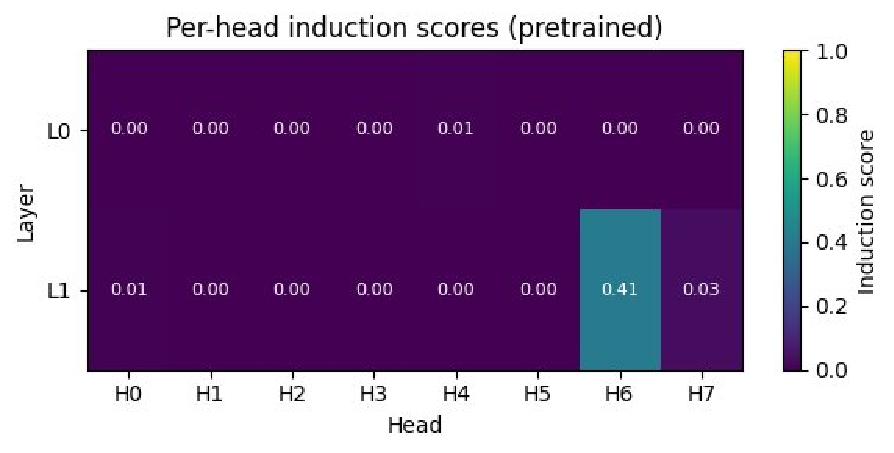
\includegraphics[width=\columnwidth]{figures/fig3_induction_scores_baseline.pdf}
  \caption{Per-head induction (prefix-matching) scores, pretrained model.
    L1H6: $0.408 \pm 0.103$; all others $< 0.034$.}
  \label{fig:ind-baseline}
\end{figure}

\begin{figure}[h]
  \centering
  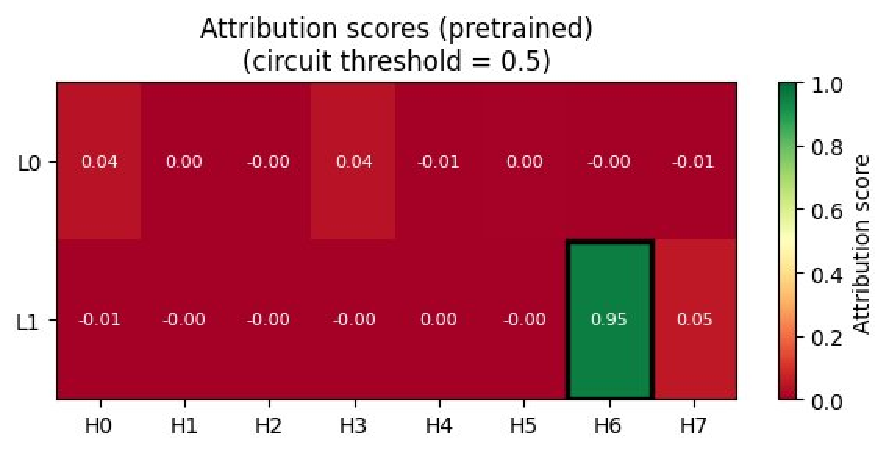
\includegraphics[width=\columnwidth]{figures/fig4_attribution_baseline.pdf}
  \caption{Activation-patching attribution, pretrained model.
    Thick border: circuit head (Attr $\geq 0.5$).
    L1H6: $0.952$; all others $< 0.053$.}
  \label{fig:attr-baseline}
\end{figure}

\begin{figure}[h]
  \centering
  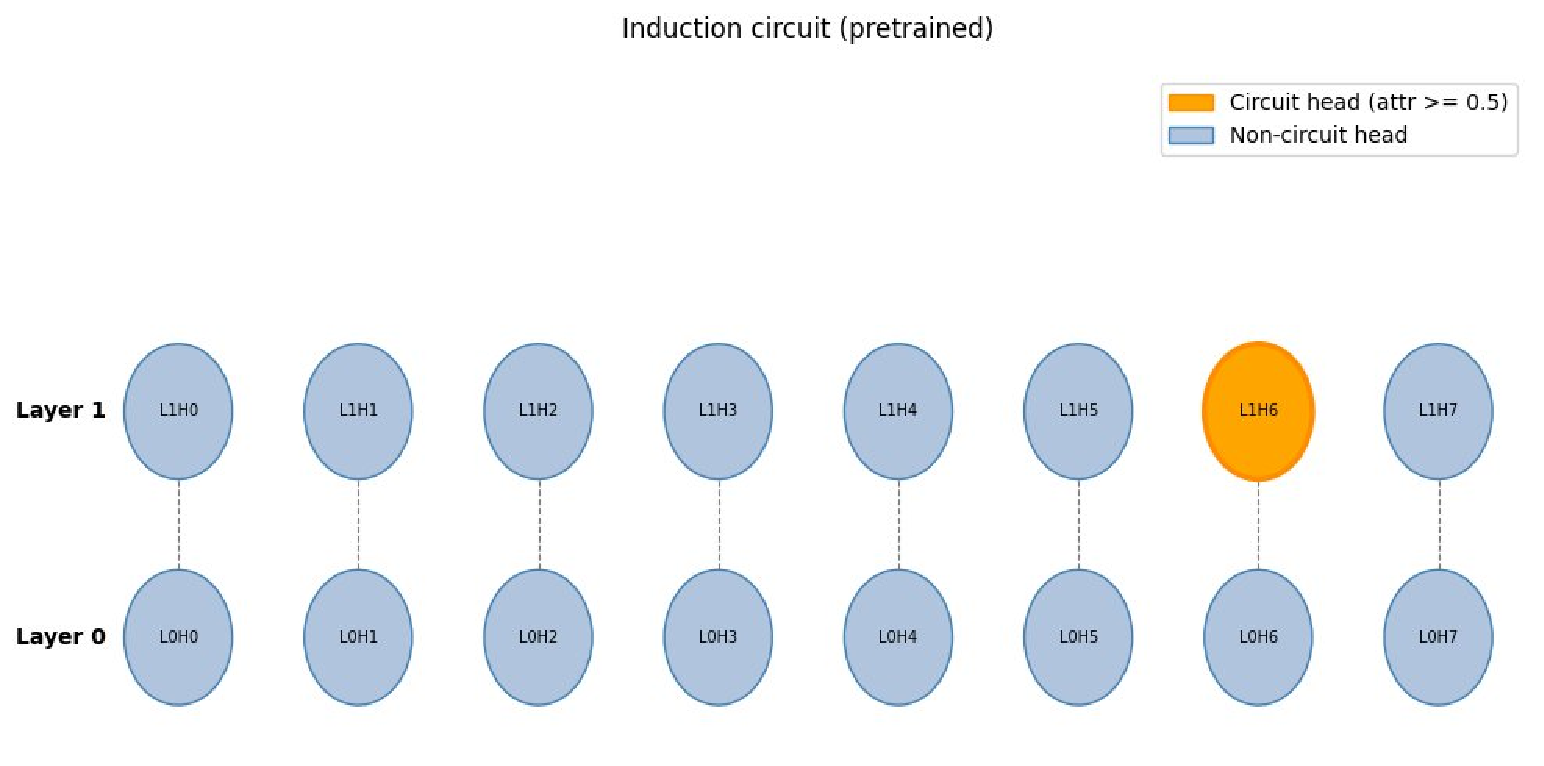
\includegraphics[width=0.85\columnwidth]{figures/fig1_circuit_diagram.pdf}
  \caption{Induction circuit diagram, pretrained model.
    L1H6 (orange) is the sole circuit member.}
  \label{fig:circuit}
\end{figure}

\begin{figure}[h]
  \centering
  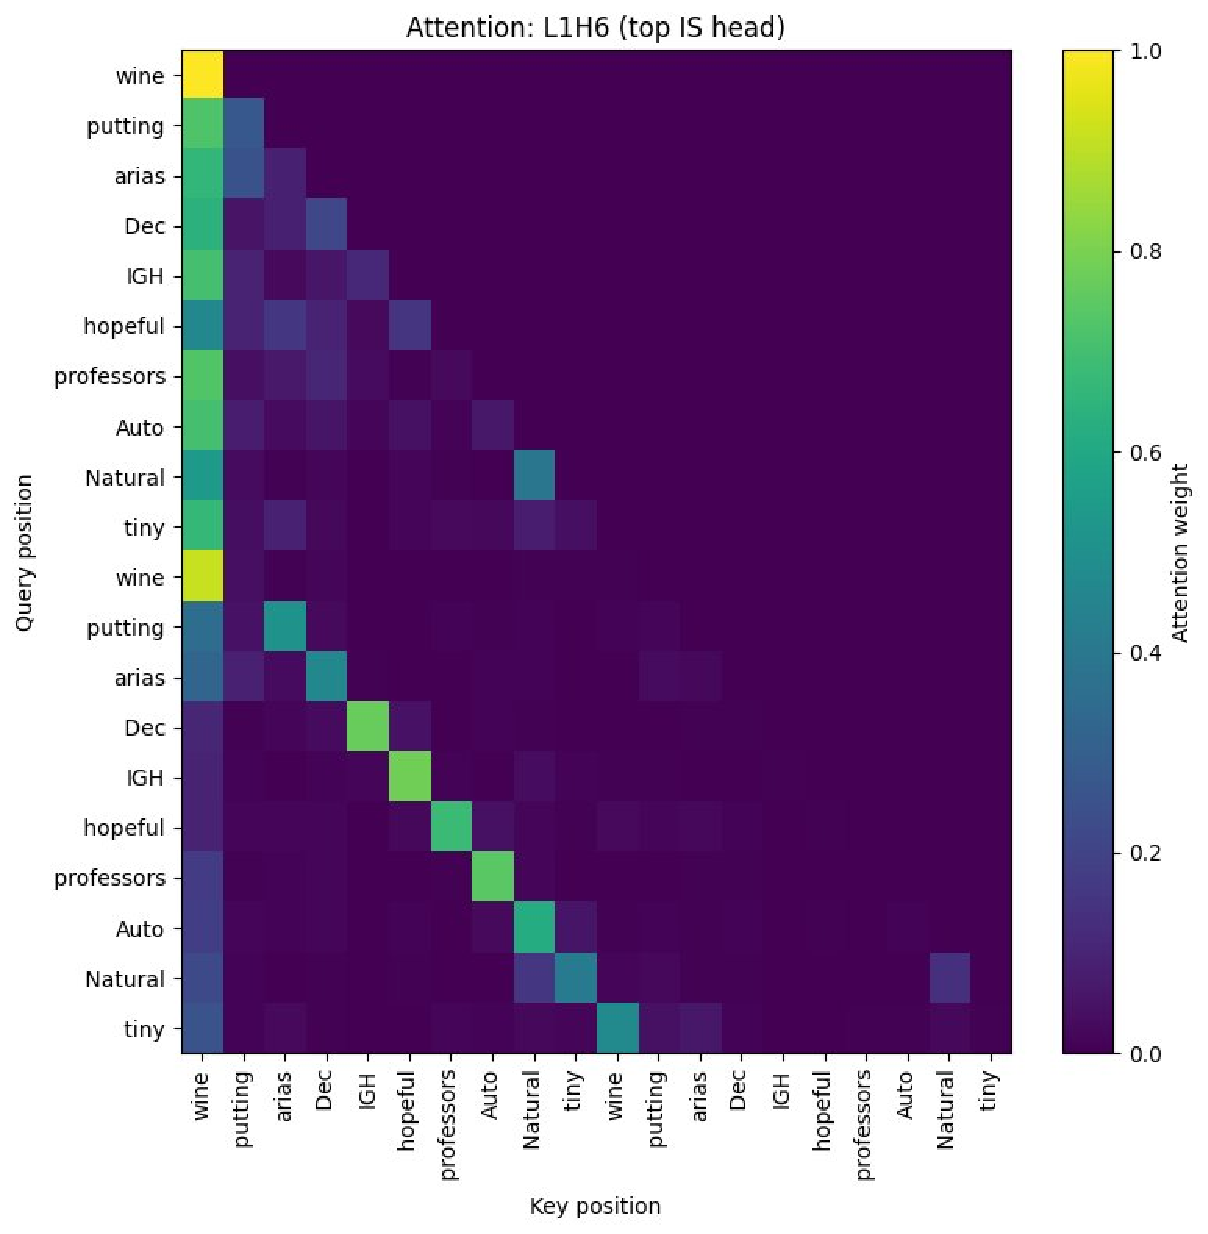
\includegraphics[width=\columnwidth]{figures/fig2_attention_heatmap.pdf}
  \caption{L1H6 attention pattern on a repeated-token sequence
    (20 tokens, period 10). The off-diagonal stripe is the
    prefix-matching pattern.}
  \label{fig:attn-heatmap}
\end{figure}

\subsection{Code Fine-Tuning}

Figure~\ref{fig:ind-code} shows L1H6's trajectory over 244 fine-tuning
steps on \texttt{transformersbook/codeparrot} (Python).
Per-head scores are from seed 42; training-loss statistics are from
all three seeds (Table~\ref{tab:main-results}).

L1H6's prefix-matching score increases monotonically:
$0.408 \to 0.584$ at step 100 ($\Delta = +0.176$) and
$0.638$ at step 200 ($\Delta_\text{cumulative} = +0.230$).
Both increments exceed the pre-registered $\geq 0.1$ meaningful-change
threshold (DECISION-004).
The IS threshold of $0.5$ is crossed between steps 0 and 100.
Concurrently, induction task cross-entropy falls from $11.848$ to $7.557$
and the clean logit difference rises from $4.631$ to $7.566$,
confirming improved task performance.

Mean training loss across three seeds at step 100:
$4.284 \pm 0.450$ (step 100), $3.181 \pm 0.965$ (step 200).
The inter-seed standard deviation is modest at step 100 and larger at
step 200, reflecting diverging loss trajectories beyond the first checkpoint.

\begin{figure}[h]
  \centering
  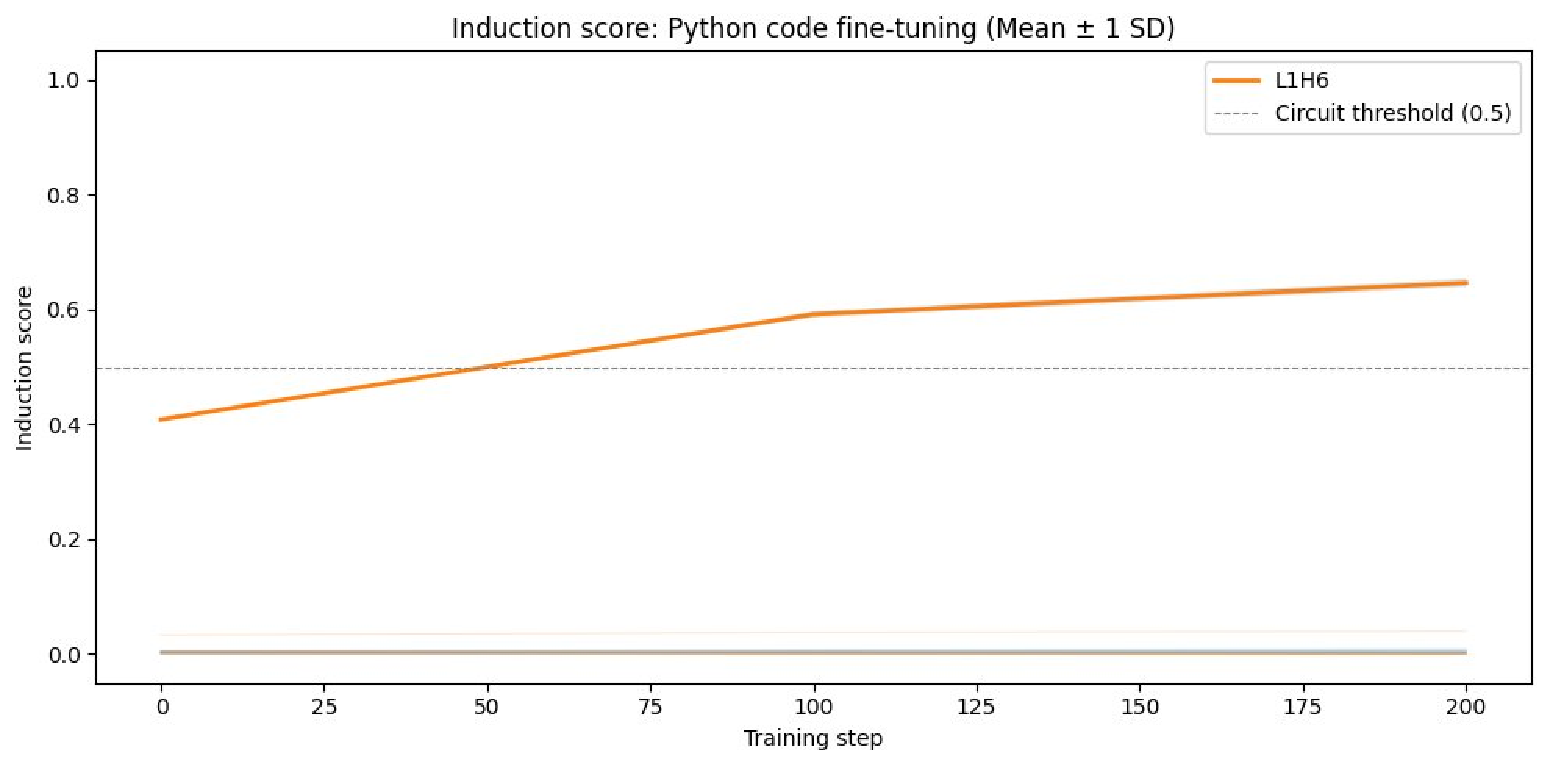
\includegraphics[width=\columnwidth]{figures/fig5_induction_code.pdf}
  \caption{L1H6 prefix-matching score vs.\ training step, Python code
    fine-tuning (seed 42). Dashed: $0.5$ IS threshold.
    Both checkpoints exceed the $\geq 0.1$ meaningful-change threshold.}
  \label{fig:ind-code}
\end{figure}

\subsection{Prose Control}

Figure~\ref{fig:ind-prose} shows the TinyStories prose control.
L1H6's score reaches $0.583$ ($\Delta = +0.175$) at step 100
and $0.616$ ($\Delta_\text{cumulative} = +0.208$) at step 200.
Mean training loss across three seeds: $4.098 \pm 0.076$ (step 100),
$3.647 \pm 0.086$ (step 200) --- notably lower inter-seed variance
than the code condition.

\begin{figure}[h]
  \centering
  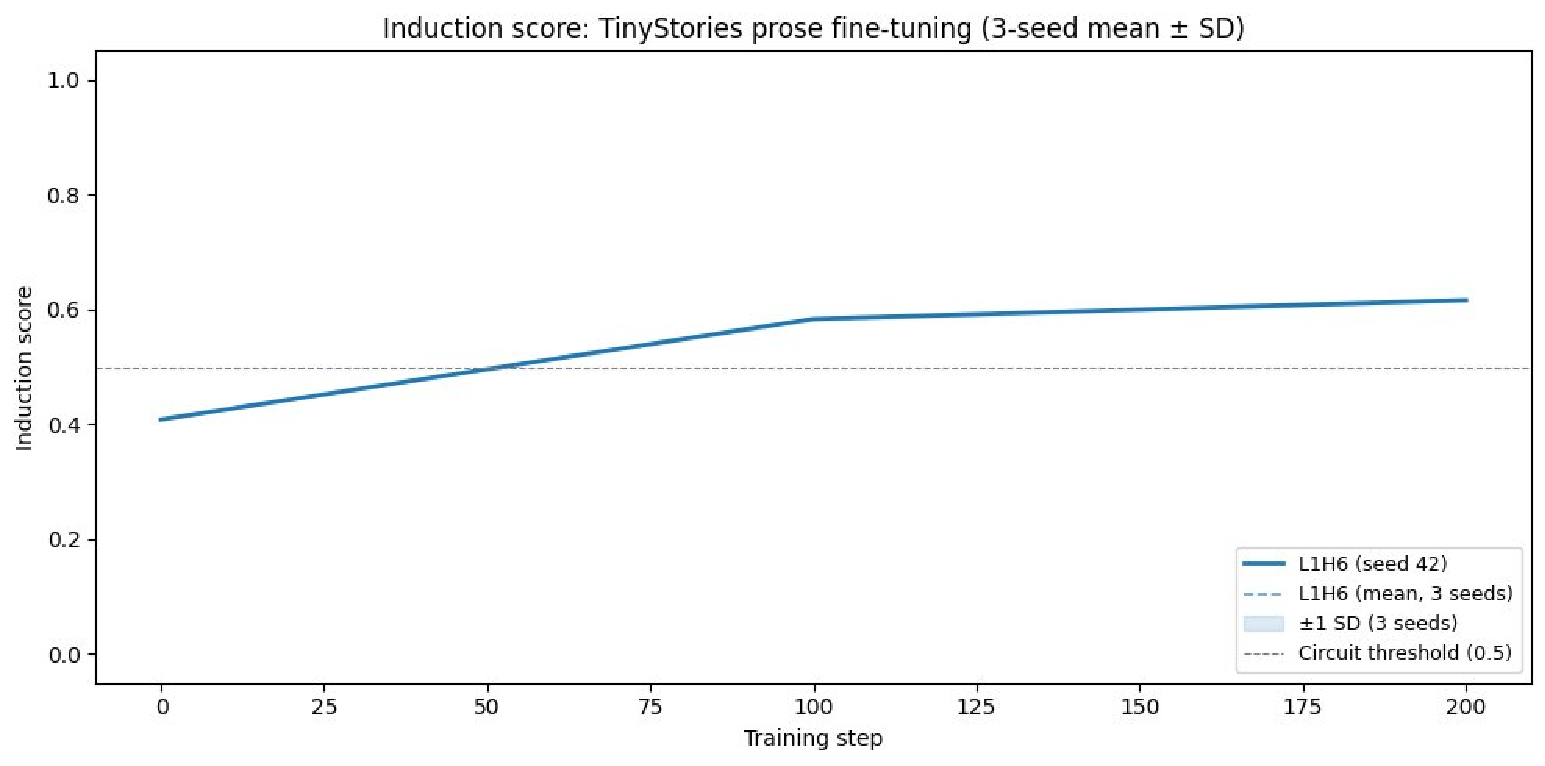
\includegraphics[width=\columnwidth]{figures/fig6_induction_prose.pdf}
  \caption{L1H6 prefix-matching score vs.\ training step,
    TinyStories prose fine-tuning (control, seed 42).
    Trajectory closely tracks the code condition.}
  \label{fig:ind-prose}
\end{figure}

\subsection{Code vs.\ Prose Comparison}

Table~\ref{tab:main-results} summarises the key metrics.
The code and prose trajectories for L1H6 are almost identical at step 100
($|\Delta\text{code} - \Delta\text{prose}| = 0.001$) and differ by only
$0.022$ at step 200.
Both conditions produce IS increases well above the $0.1$ threshold and
neither shows dissolution.
At single-seed, 3-checkpoint resolution, these differences are not
statistically discriminable; completing the per-head sweep for seeds 123
and 7 (checkpoints exist) is the next step.

\begin{table}[h]
\centering
\footnotesize
\begin{tabular}{lccccc}
\toprule
\multirow{2}{*}{Condition} & \multirow{2}{*}{Step} &
\multirow{2}{*}{L1H6 IS} & \multirow{2}{*}{$\Delta$ IS} &
\multicolumn{2}{c}{Train loss (3 seeds)} \\
\cmidrule(lr){5-6}
& & & & Mean & SD \\
\midrule
Pretrained & 0   & $0.408$ & ---       & ---   & --- \\
\midrule
Code  & 100 & $0.584$ & $+0.176$ & $4.284$ & $0.450$ \\
Code  & 200 & $0.638$ & $+0.230$ & $3.181$ & $0.965$ \\
\midrule
Prose & 100 & $0.583$ & $+0.175$ & $4.098$ & $0.076$ \\
Prose & 200 & $0.616$ & $+0.208$ & $3.647$ & $0.086$ \\
\bottomrule
\end{tabular}
\caption{L1H6 prefix-matching score (seed 42) and training loss
  (mean $\pm$ SD over 3 seeds) at each checkpoint.
  IS values are from seed 42 only; train-loss statistics use all three seeds.}
\label{tab:main-results}
\end{table}

\subsection{Phase Transition Analysis}

Figure~\ref{fig:phase} shows L1H6's trajectory with the detected
transition. A single transition exceeding the $0.1$ threshold is detected
at step 100 in both conditions (Table~\ref{tab:phase}).
No transition is detected between steps 100 and 200
($|\Delta| = 0.054$ code, $0.033$ prose), consistent with a front-loaded
increase followed by a partial plateau.

\begin{table}[h]
\centering
\begin{tabular}{lcccc}
\toprule
Condition & Step & IS before & IS after & $\Delta$ \\
\midrule
Code  & 100 & $0.408$ & $0.584$ & $+0.176$ \\
Prose & 100 & $0.408$ & $0.583$ & $+0.175$ \\
\bottomrule
\end{tabular}
\caption{Detected phase transitions for L1H6 ($|\Delta| \geq 0.1$,
  seed 42). No other head crosses the threshold in either condition.}
\label{tab:phase}
\end{table}

\begin{figure}[h]
  \centering
  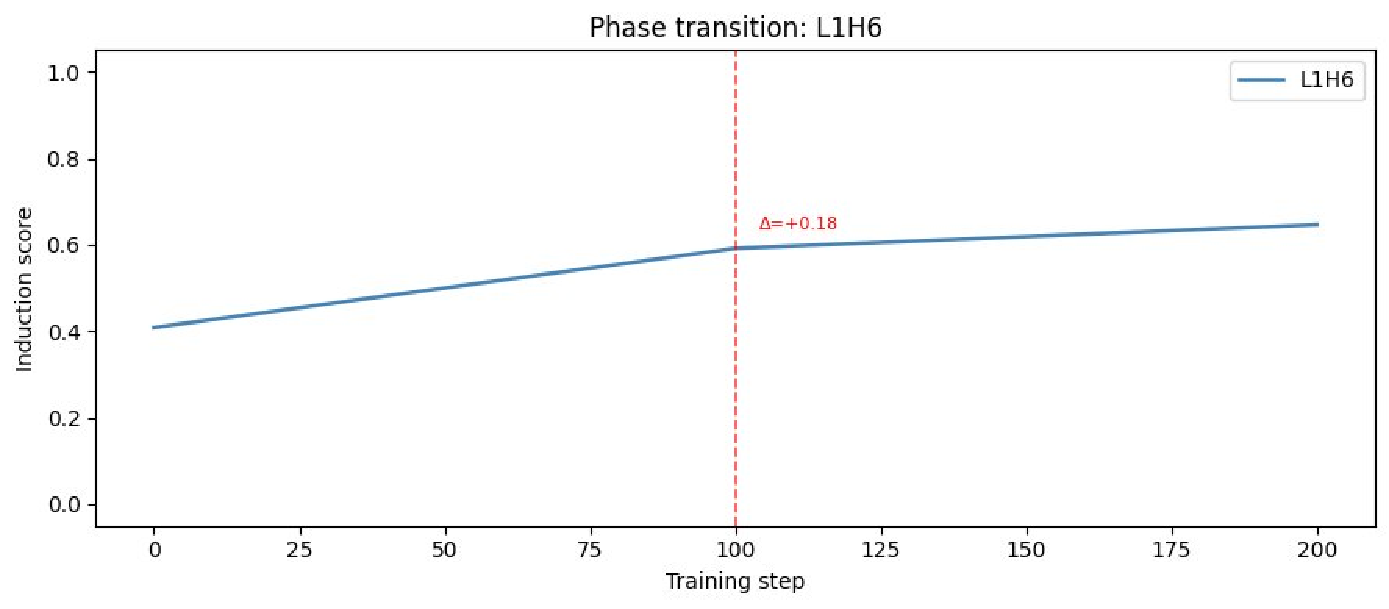
\includegraphics[width=\columnwidth]{figures/fig7_phase_transition.pdf}
  \caption{Phase transition for L1H6, code fine-tuning (seed 42).
    Red dashed: detected transition at step 100 ($\Delta = +0.176$).}
  \label{fig:phase}
\end{figure}

\subsection{Adversarial Probes}

Figure~\ref{fig:adv} and Table~\ref{tab:adv} show the 22-probe
adversarial results for the post-fine-tuning model (code, step 200).

\textbf{Structure-preserving probes} (\texttt{sub\_pos\_*},
\texttt{sub\_end\_*}, \texttt{multi\_sub\_*}, \texttt{clean\_repeated}):
post mean $= 0.944 \pm 0.043$, essentially unchanged from pre
($0.941 \pm 0.047$). The circuit is robust to minor perturbations.

\textbf{Structure-removing probes} (\texttt{reversed\_second\_half},
\texttt{cyclic\_shift\_1/3}, \texttt{fully\_random}):
post mean $= 0.132 \pm 0.030$, confirming the head is selective
to prefix-matching structure and not a generic high-attention bias.

\textbf{Competing-pattern probes} (\texttt{competing\_a/b},
\texttt{long\_lag\_2/3}): post mean $= 0.355 \pm 0.122$,
reflecting partial but not full induction under competing stimuli.

\textbf{Degenerate case} (\texttt{all\_same\_token}):
pre $= 4.123$, post $= 2.414$ ($\Delta = -1.709$).
This probe is a normalisation artefact (all positions trivially satisfy
the criterion simultaneously); its large \emph{decrease} post fine-tuning
indicates the circuit becomes more discriminating, not more susceptible
to degenerate inputs (see Section~\ref{sec:limitations}).

\begin{table}[h]
\centering
\begin{tabular}{lccc}
\toprule
Category & $n$ & Pre & Post \\
\midrule
Structure-preserving  & 13 & $0.941 \pm 0.047$ & $0.944 \pm 0.043$ \\
Structure-removing    &  4 & $0.162 \pm 0.029$ & $0.132 \pm 0.030$ \\
Competing patterns    &  4 & $0.357 \pm 0.106$ & $0.355 \pm 0.122$ \\
\texttt{all\_same\_token} (degenerate) & 1 & $4.123$ & $2.414$ \\
\bottomrule
\end{tabular}
\caption{Adversarial probe results by category (mean $\pm$ SD within
  category; degenerate probe separate; $n=22$ probes total).
  Post = code fine-tuning, seed 42, step 200.}
\label{tab:adv}
\end{table}

\begin{figure}[h]
  \centering
  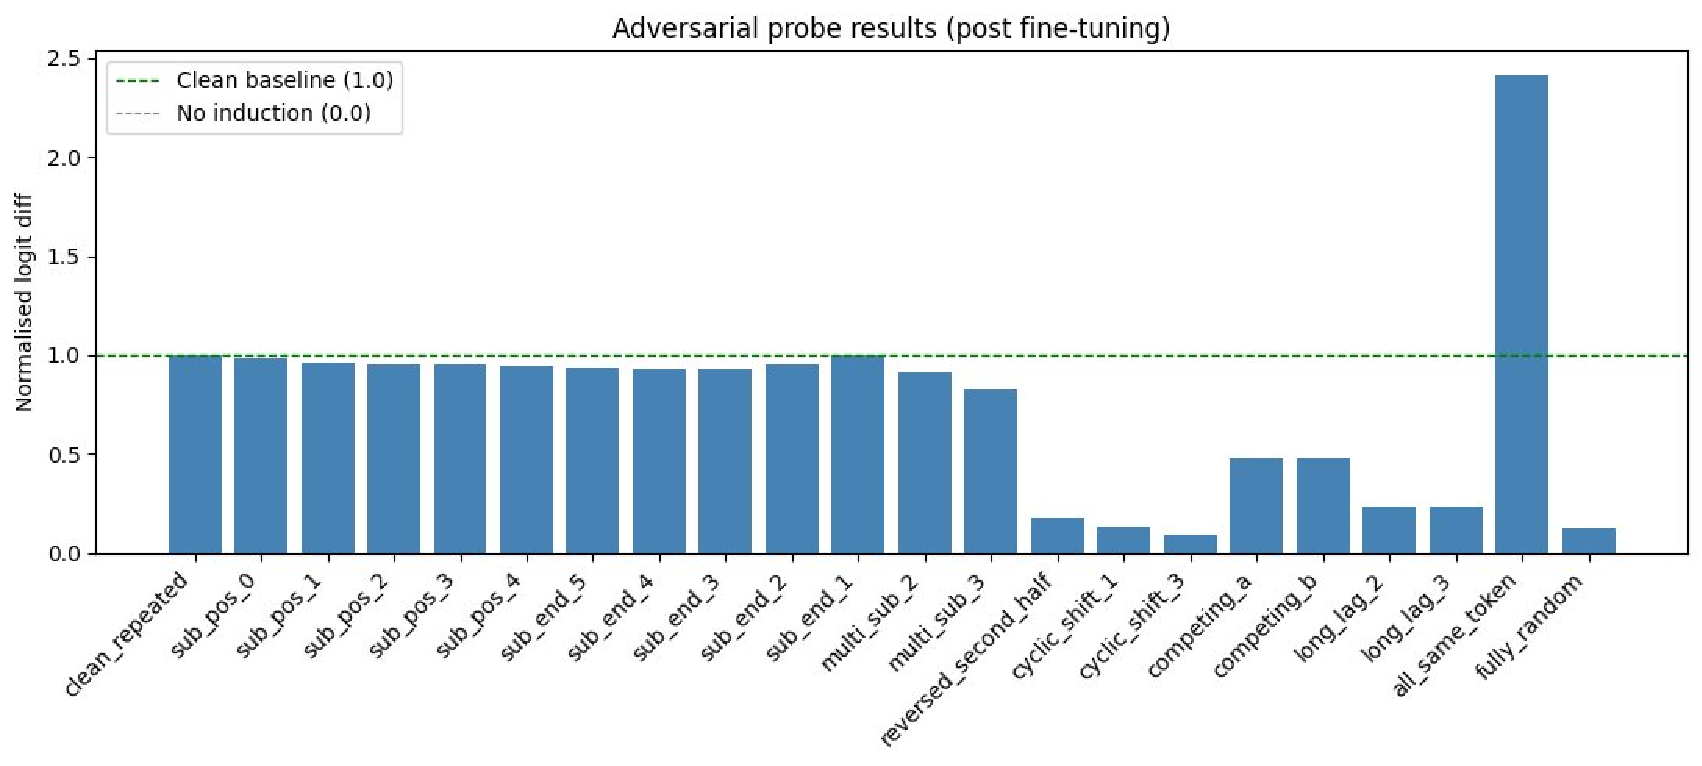
\includegraphics[width=\columnwidth]{figures/fig8_adversarial.pdf}
  \caption{Adversarial probe results, post fine-tuning (code, seed 42,
    step 200). Dashed green: clean baseline (1.0).
    Dashed grey: no-induction reference (0.0).
    \texttt{all\_same\_token} bar ($= 2.41$) truncated; see
    Section~\ref{sec:limitations}.}
  \label{fig:adv}
\end{figure}
